
\begin{frame}
	\titre{Intro à Port-Royal}
	
	\begin{description}[labelindent=6pt,style=multiline,leftmargin=1.3in]
		 \setlength\itemsep{1.4em}
		 
		 \item[Qui] Antoine Arnauld et Pierre Nicole
		 \pause
		 \item[Où] L'abbaye de Port-Royal (rien à voir avec le métro), haut lieu du jansénisme à l'époque
		 \pause
		 \item[Quand] 1662
		 \pause
		 \item[Quoi] Le bouquin `La logique ou l'art de penser`
		 
	\end{description}
\end{frame}



\begin{frame}
	\titre{Intro à Port-Royal}
	
	\begin{description}[labelindent=6pt,style=multiline,leftmargin=1.3in]
		 \setlength\itemsep{1.4em}
		 
		 \item[But] Distinguer les bons des mauvais syllogismes
		 \pause
		 \item[] C'est à dire ceux qui sont \textbf{valides} et ceux qui ne le sont pas
		 \pause
		 \item[Problème] Y a du travail
		 \pause
		 \item[`Solution`] \textit{Fixer avec précision l'objet d'étude} \pause (cad se resteindre à un chantier plus simple) \pause
		 \item On s'intéresse uniquement aux raisonnements avec 2 prémisses + 1 conclusion\pause, le tout quantifié
 		 
	\end{description}
\end{frame}



\begin{frame}
	\titre{Intro à Port-Royal}
	
	\begin{description}[labelindent=6pt,style=multiline,leftmargin=1.3in]
		 \setlength\itemsep{1em}
		 
		 \item[Rappel] Les \textit{termes} utilisés dans un raisonnement n'ont pas (vraiment) d'importance
		 \pause
		 \item[] \begin{tabular}{l}
Tous les alcooliques sont bigleux\\
Tous les bigleux sont blonds\\ \cline{1-1}
Tous les alcooliques sont blonds\\
\end{tabular}
		 \item[$\equiv$] \begin{tabular}{l}
Tous les barmans sont chauves\\
Tous les chauves sont méchants\\ \cline{1-1}
Tous les barmans sont méchants\\
\end{tabular}\pause


		 \item[$\equiv$] \begin{tabular}{l}
Tous les X sont Y\\
Tous les Y sont Z\\ \cline{1-1}
Tous les X sont Z\\
\end{tabular}
	\end{description}
\end{frame}


\begin{frame}
	\titre{Intro à Port-Royal}
	
	\begin{description}[labelindent=6pt,style=multiline,leftmargin=1.3in]
		 \setlength\itemsep{1em}
		 
		 \item[Idée] On peut donc espérer \textit{énumérer} (lister) l'ensemble des \textbf{schémas} possibles si on trouve les \textbf{paramètres} pertinents
		 \pause
		 \item[Définition] Les conclusions seront de la forme 
\begin{tabular}[t]{clc}
B &est& A\\
\textbf{petit terme} &&\textbf{grand terme}\\
\end{tabular}
 \pause
		 \item[Définition] Pour répondre à la question, on va passer par un autre terme, le \textbf{moyen}
\pause

		 \item[]
\begin{tabular}{cccl}
A  & $\leftrightarrow$ & M & (prémisse) majeure\\
M  & $\leftrightarrow$ & B & (prémisse) mineure\\
\hline
B  & est & A & conclusion\\
\end{tabular}
	\end{description}
\end{frame}


\begin{frame}
	\titre{Figures}
	
	\begin{description}[labelindent=6pt,style=multiline,leftmargin=1.3in]
		 \setlength\itemsep{1em}
		 
		 \item[]
\begin{tabular}{cccl}
A  & $\leftrightarrow$ & M & (prémisse) majeure\\
M  & $\leftrightarrow$ & B & (prémisse) mineure\\
\hline
B  & est & A & conclusion\\
\end{tabular}

\item[Remarque] L'ordre peut changer (d'où les $\leftrightarrow$)\pause, pour un total de 4 combinaisons
\pause
\item[Constantes] A (grand terme) = attribut de la conclusion \pause
\item[] B (petit terme) = sujet de la conclusion \pause 
\item[] M (moyen) = attribut ou sujet \newline \pause 
	\end{description} 

	Majeure (resp. Mineure) = prémisse impliquant le grand (resp. petit) terme 
\end{frame}




\begin{frame}
	\titre{Figures}
	
	\begin{tabular}{ccc}
\begin{tabular}{lcc}
1\iere\ figure	& M & A \\
		& B & M \\
\cline{2-3}
		& B & A \\
\end{tabular}
%

&
\textcolor{white}{lolilol}
&
\begin{tabular}{lcc}
2\ieme\ figure	& A & M \\
		& B & M \\
\cline{2-3}
		& B & A \\
\end{tabular} \\
%


\textcolor{white}{lolilol} & 
\textcolor{white}{lolilol} & 
\textcolor{white}{lolilol} \\


\textcolor{white}{lolilol} & 
\textcolor{white}{lolilol} & 
\textcolor{white}{lolilol} \\


\textcolor{white}{lolilol} & 
\textcolor{white}{lolilol} & 
\textcolor{white}{lolilol} \\

\begin{tabular}{lcc}
3\ieme\ figure	& M & A \\
		& M & B \\
\cline{2-3}
		& B & A \\
\end{tabular}

&
\textcolor{white}{lolilol}
&
\begin{tabular}{lcc}
4\ieme\ figure	& A & M \\
		& M & B \\
\cline{2-3}
		& B & A \\
\end{tabular}
\end{tabular}
\end{frame}



\begin{frame}
	\titre{Modes}
	
	\begin{description}[labelindent=6pt,style=multiline,leftmargin=1.3in]
		 \setlength\itemsep{1em}

\item[Mode] Arrangement de 3 propositions ayant 4 formes possibles (A, I, E ou O) \pause $\rightarrow$ 64 combinaisons (AAA, EIO, AEE, etc ...)\pause
\item[] On va pouvoir combiner figure et mode \pause : si le mode est $Q_1Q_2Q_3$, la grand prémisse sera $Q_1$, la petite sera $Q_2$ et la conclusion sera $Q_3$. \pause
\item[But du jeu] Essayer toutes les figures avec tous les modes \pause pour un total de 256 syllogismes à tester ! 

	\end{description} 
\end{frame}



\begin{frame}
	\titre{C'est parti ! (1/256)}
	
	\begin{description}[labelindent=6pt,style=multiline,leftmargin=1.3in]
		 \setlength\itemsep{1em}

\item[$3^{\grave{e}me}$ figure] \begin{tabular}{cc}
M & A \\
	M & B \\
\cline{1-2}
		B & A \\
\end{tabular}
\item[Mode] AAA \pause
\item[Attention] Les `A` du mode et ceux de la figure n'ont rien à voir ! \pause (personne n'a dit que le formalisme était bien foutu) \pause
\item[Question] Valide ? 

	\end{description} 
\end{frame}



\begin{frame}
	\titre{C'est parti ! (1/256)}
	
	\begin{description}[labelindent=6pt,style=multiline,leftmargin=1.3in]
		 \setlength\itemsep{1em}

\item[Mode + figure] \begin{tabular}{c}
Tous les M sont A\\ 
Tous les M sont B\\ 
\cline{1-1}
Tous les B sont A
\end{tabular} \pause
\item[Explication] On peut imaginer un monde dans lequel il y a uniquement 2 individus, Jean-Michel qui est à la fois M, A et B, et Jean-Charles qui est uniquement B \pause
\item[] Les deux \textbf{hypothèses} sont \textbf{respectées} (tout M est également A et B), mais la \textbf{conclusion} est \textbf{fausse} (JC l'enfreint)\pause
\item[Réponse] Pas valide, car on a un \textbf{contre-exemple} 

	\end{description} 
\end{frame}


\begin{frame}
	\titre{C'est parti ! (1/256)}
	
	\begin{description}[labelindent=6pt,style=multiline,leftmargin=1.3in]
		 \setlength\itemsep{1em}

\item[Mode + figure] \begin{tabular}{c}
Tous les M sont A\\ 
Tous les M sont B\\ 
\cline{1-1}
Tous les B sont A
\end{tabular}
\item[Explication] On peut imaginer un monde dans lequel il y a uniquement 2 individus, Jean-Michel qui est à la fois M, A et B, et Jean-Charles qui est uniquement B
\item[Remarque] Un truc à dire sur ce contre-exemple \only<1>{? \textcolor{white}{pour l'améliorer}}\only<2->{pour l'améliorer ?}\pause  \pause
\item[] Il n'est pas minimal\pause, on peut se passer de Jean-Michel

	\end{description} 
\end{frame}



\begin{frame}
	\titre{Méthodologie}
	
	\begin{description}[labelindent=6pt,style=multiline,leftmargin=1.3in]
		 \setlength\itemsep{1em}
		 
\item[Remarque] \textbf{Un (contre-)exemple sert uniquement à montrer qu'un syllogisme n'est pas valide} \pause
\item[] On pourrait aussi imaginer un monde où il y a un seul individu, qui est M, A et B\pause
\item[] Dans ce cas, hypothèses + conclusion respectées\pause
\item[] Le syllogisme n'en est pas pour autant valide !
\item[] Pour montrer la validité, ça va donc être un peu plus abstrait 
	\end{description} 

	
\end{frame}

\begin{frame}
	\titre{Méthodologie}
	
	\begin{description}[labelindent=6pt,style=multiline,leftmargin=1.3in]
		 \setlength\itemsep{1em}
		 
\item[Par contre] Les contre-exemples se présentent très bien sous la forme de \textbf{diagrammes de Venn} (aussi appelés patatoïdes)\pause
\item[Exemple] 	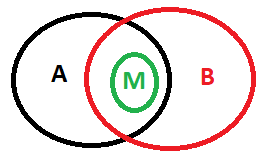
\includegraphics[scale=0.5]{1256.png}\pause
\item[] Chaque \textit{patate} représente l'ensemble des individus qui ont la propriété associée\pause
\item On a bien les hypothèses respectées et la conclusion falsifiée
	\end{description} 

	
\end{frame}







%
%\begin{frame}
%	\titre{C'est parti ! (1/256 prise 2)}
%	
%	\begin{description}[labelindent=6pt,style=multiline,leftmargin=1.3in]
%		 \setlength\itemsep{1em}
% 
%\item[Exemple] 
%\begin{tabular}{c}
%Tous les canards sont mexicains \\
%	Tous les canards jouent au poker \\
%\cline{1-1}
%Tous les joueurs de poker sont mexicains \\
%\end{tabular}
%\pause
%\item[Explication] Soit un monde dans lequel tous les canards sont des joueurs de poker mexicains, et Jean-Luc un joueur de poker non-canard, non-mexicain. Aucune des hypothèses n'est violée, tandis que la conclusion n'est pas vraie. \pause
%\item[Réponse] Pas valide, car on a un \textbf{contre-exemple} 
%	\end{description} 
%\end{frame}
%


\begin{frame}
	\titre{C'est parti ! (2/256)}
	
	\begin{description}[labelindent=6pt,style=multiline,leftmargin=1.3in]
		 \setlength\itemsep{1em}

\item[$1^{\grave{e}re}$ figure] \begin{tabular}{cc}
M & A \\
	B & M \\
\cline{1-2}
		B & A \\
\end{tabular}
\item[Mode] AAA \pause
\item[Question] Valide ? 

	\end{description} 
\end{frame}



\begin{frame}
	\titre{C'est parti ! (2/256)}
	
	\begin{description}[labelindent=6pt,style=multiline,leftmargin=1.3in]
		 \setlength\itemsep{1em}

\item[Mode + figure] \begin{tabular}{c}
Tous les M sont A\\ 
Tous les B sont M\\ 
\cline{1-1}
Tous les B sont A
\end{tabular} \newline
	\end{description}
	
Prenons un B \textbf{arbitraire}\pause, cad sur lequel on n'a aucune autre information \pause
\newline 

La prémisse min. nous dit qu'il est aussi M\pause
\newline

La prémisse maj. nous dit alors qu'il est aussi A\pause \newline

Syllogisme valide \pause : on a montré qu'un individu, \textbf{dont on savait seulement qu'il était B}, est aussi un A. \pause Ca prouve que \textbf{n'importe quel B} sera aussi A

\end{frame}


\begin{frame}
	\titre{C'est parti ! (2/256 prise 2)}
	
	\begin{description}[labelindent=6pt,style=multiline,leftmargin=1.3in]
		 \setlength\itemsep{1em}

\item[Mode + figure] \begin{tabular}{c}
Tous les M sont A\\ 
Tous les B sont M\\ 
\cline{1-1}
Tous les B sont A
\end{tabular} \newline
	\end{description}
	
	 
Prenons un B \textbf{arbitraire}, cad sur lequel on n'a aucune autre information \pause \newline 

La prémisse min. permet de le \textbf{transformer} en M\pause \newline

La prémisse maj. permet de \textbf{transformer} le M obtenu en A \pause \newline

Syllogisme valide \pause : on a montré qu'en \textbf{composant} (combinant) les deux prémisses, on crée \only<1-4>{\textcolor{white}{une \textit{méthode}}}\only<5>{une \textit{méthode}}\only<6>{une \textit{fonction}}\only<7>{un \textbf{programme}} permettant de \textbf{transformer} tout B en A \pause

\end{frame}


%
%\begin{frame}
%	\titre{Méthodo validité}
%	
%Dans le cas d'une démonstration de non-validité d'un syllogisme, vous pouvez utiliser des exemples `concrets` ou rester abstrait, selon ce avec quoi vous êtes le plus à l'aise \newline
%\pause
%
%La non-importance des termes fait que vous pourriez théoriquement avoir le même choix au moment de prouver la validité d'un syllogisme\pause, mais pour vous faire prendre des bonnes habitudes, on va se limiter à l'abstrait \newline
%
%\pause
%En maths, un \textbf{exemple} ne prouve pas un résultat \textit{général}. Ici c'est un cas un peu dégénéré qu'on va donc ignorer.
%
%\end{frame}


\begin{frame}
	\titre{La slide barbante}
	
Vous pouvez choisir d'utiliser le style `$x$ est un A et telle prémisse nous dit que tout A est aussi un M, donc $x$ est un M`\pause, ou `x est un A et telle prémisse permet de \textit{transformer} tout A en M, donc on peut faire de x un M`. \newline \pause

La différence n'est sans doute pas évidente, mais représente les deux (grosses) approches des fondements des mathématiques ! \pause \newline

Le premier style correspond à un point de vue \textbf{théorie des ensembles} (patatoïdes), tandis que la deuxième formulation découle de la \textbf{théorie des types} (programmes). \pause Le schisme entre ces deux théories est une conséquence du \textbf{paradoxe de Russel} (1901$\sim$1903).

\end{frame}



\begin{frame}
	\titre{C'est (re-)parti ! (3/256)}
	
	\begin{description}[labelindent=6pt,style=multiline,leftmargin=1.3in]
		 \setlength\itemsep{1em}

\item[$2^{\grave{e}me}$ figure] \begin{tabular}{cc}
A & M \\
	B & M \\
\cline{1-2}
		B & A \\
\end{tabular}
\item[Mode] AAI \pause
\item[Question] Valide ? 

	\end{description} 
\end{frame}



\begin{frame}
	\titre{C'est (re-)parti ! (3/256)}
	
	\begin{description}[labelindent=6pt,style=multiline,leftmargin=1.3in]
		 \setlength\itemsep{1em}

\item[Mode + figure] \begin{tabular}{c}
Tous les A sont M\\ 
Tous les B sont M\\ 
\cline{1-1}
Certains B sont A
\end{tabular}\pause
\item[Explication] On peut imaginer un monde dans lequel il y a seulement 2 individus : Jean-Michel qui est à la fois A et M, et Jean-Charles qui est uniquement B et M\pause
\item[] Les deux hypothèses sont respectées (tout individu A ou B est également M), mais la conclusion est fausse (le seul B n'est pas A)\pause
\item[Réponse] Pas valide, car on a un \textbf{contre-exemple} 

	\end{description} 
\end{frame}


\begin{frame}
	\titre{C'est (re-)parti ! (3/256 bonus)}
	
	\begin{description}[labelindent=6pt,style=multiline,leftmargin=1.3in]
		 \setlength\itemsep{1em}

\item[AAX + fig. 3] \begin{tabular}{c}
Tous les A sont M\\ 
Tous les B sont M\\ 
\cline{1-1}
[relation entre A et B]
\end{tabular} \pause
\item[Remarque] Etant donnée la figure, aucun mode de la forme AAX ne sera valide
\pause
\item[] En effet, imaginez que M est l'ensemble des individus\pause, alors les deux prémisses deviennent `tous les individus ayant la prop A (ou B) sont des individus`\pause
\item[] Ca n'apporte strictement aucune information, on ne va rien pouvoir conclure

	\end{description} 
\end{frame}






\begin{frame}
	\titre{C'est (re-)parti ! (7/256)}
	
	\begin{description}[labelindent=6pt,style=multiline,leftmargin=1.3in]
		 \setlength\itemsep{1em}

\item[$1^{\grave{e}re}$ figure] \begin{tabular}{cc}
M & A \\
	B & M \\
\cline{1-2}
		B & A \\
\end{tabular}
\item[Mode] III \pause
\item[Question] Valide ? 

	\end{description} 
\end{frame}



\begin{frame}
	\titre{C'est (re-)parti ! (7/256)}
	
	\begin{description}[labelindent=6pt,style=multiline,leftmargin=1.3in]
		 \setlength\itemsep{1em}

\item[Mode + figure] \begin{tabular}{c}
Certains M sont A\\ 
Certains B sont M\\ 
\cline{1-1}
Certains B sont A
\end{tabular}\pause
\end{description}
\only<1>{\vspace{5cm}}
\only<2-3>{
	\begin{description}[labelindent=6pt,style=multiline,leftmargin=1.3in]
		 \setlength\itemsep{1em}
\item[Contre-ex] On a 10 individus $p_1$ à $p_{10}$. $p_1$ est M et A (et pas B), $p_2$ est B et M (et pas A), le reste n'est jamais A et B à la fois\pause
\item[] Les deux hypothèses sont respectées (grâce à $p_1$ et $p_2$), mais la conclusion est fausse (peut se vérifier sur chaque individu)\pause
\end{description}
\vspace{1.47cm}
}

\only<4>{
	\vspace{1.2cm}
	\begin{figure}[H]
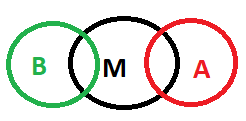
\includegraphics[scale=0.5]{4256.png}
\end{figure}\vspace{1.9cm}}

\pause

\only<5>{
	\vspace{1.2cm}
	\begin{figure}[H]
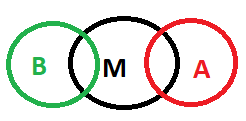
\includegraphics[scale=0.5]{4256.png}
\end{figure}
	\begin{description}[labelindent=6pt,style=multiline,leftmargin=1.3in]
		 \setlength\itemsep{1em}
\item[Réponse] Pas valide, car on a un \textbf{contre-exemple} 
	\vspace{1.1cm}
	\end{description}}

	 
\end{frame}



\begin{frame}
	\titre{C'est (re-)parti ! (7/256)}
	
	\begin{description}[labelindent=6pt,style=multiline,leftmargin=1.3in]
		 \setlength\itemsep{1em}

\item[Mode + figure] \begin{tabular}{c}
Certains M sont A\\ 
Certains B sont M\\ 
\cline{1-1}
Certains B sont A
\end{tabular}
	\end{description} 
De façon générale, on ne pourra jamais rien tirer de deux propositions particulières\pause \newline

Quel que soit le type (A / E / I / O) de la conclusion, on pourra créer une situation qui valide les deux hypotheses (particulières) sans valider la conclusion (comme on vient de le faire)\pause \newline

En fait, pas mal de règles de ce type, qui réduisent l'ensemble des syllogisme à tester, ont été identifiées.


\end{frame}
	


\begin{frame}
	\titre{Règles de base des syllogismes}
	
	\begin{itemize}
	
	\item[1] Le moyen doit être pris au moins une fois universellement\pause
	\item[2]   Les termes de la conclusion ne peuvent point être pris plus universellement dans la conclusion que dans les prémisses\pause
	\item[3]  On ne peut rien conclure de deux propositions négatives\pause
	\item[4]  On ne peut prouver une conclusion négative par deux propositions affirmatives\pause
	\item[5]  La conclusion suit toujours la plus faible partie, cad que s'il y a une des deux propositions négatives, elle est négative, et s'il y en a une particulière, elle doit être particulière\pause
	\item[6]  De deux propositions particulières il ne s'ensuit rien
	
	\end{itemize}
	
\end{frame}
	


\begin{frame}
	\titre{Pause discussion}
	
	\begin{description}[labelindent=6pt,style=multiline,leftmargin=1.3in]
		 \setlength\itemsep{1em}

\item[Remarques] ?\pause
\item[Pts positifs] Différence vérité / validité\pause
\item[] Début de classification ...\pause
\item[Pts négatifs] ... un peu bancale ...\pause
\item[] ... et arbitraire\pause
\item[] Système très \textbf{incomplet} (les propositions valides ne sont pas toutes couvertes) ... \pause
\item[] ... et pourtant redondant (cf A / E / I / O)
\end{description}
\end{frame}
	
	

% 6/256

\begin{frame}
	\titre{C'est (re-)parti ! (?/256)}
	
	\begin{description}[labelindent=6pt,style=multiline,leftmargin=1.3in]
		 \setlength\itemsep{1em}

\item[$4^{\grave{e}me}$ figure] \begin{tabular}{ll}
A & M \\
	M & B \\
\cline{1-2}
		B & A \\
\end{tabular}
\item[Mode] EAO \pause
\item[Question] Valide ? 

	\end{description} 
\end{frame}



\begin{frame}
	\titre{C'est (re-)parti ! (?/256)}
	
	\begin{description}[labelindent=6pt,style=multiline,leftmargin=1.3in]
		 \setlength\itemsep{1em}

\item[Mode + figure] \begin{tabular}{l}
Aucun A n'est M\\ 
Tous les M sont B\\ 
\cline{1-1}
Certains B ne sont pas A
\end{tabular} \newline
	\end{description} \pause
Quand on a une conclusion négative, c'est souvent plus simple de raisonner par l'absurde\pause \newline

On part du principe (potentiellement abusivement ...) que toute propriété est soit fausse, soit vraie.\newline \pause

Si on prouve qu'elle ne peut pas être fausse, elle doit donc forcément être vraie. \pause On va donc supposer qu'elle est fausse, et voir si ça introduit un paradoxe, auquel cas on a gagné.
\end{frame}


\begin{frame}
	\titre{C'est (re-)parti ! (?/256)}
	
	\begin{tabular}{l}
\textcolor{green}{Aucun A n'est M}\\ 
\textcolor{red}{Tous les M sont B}\\ 
\textcolor{blue}{Tous les B sont A}\\ 
\cline{1-1}
[Paradoxe, fin du monde, invasion de sauterelles] \\
\textcolor{white}{lol}
\end{tabular} \newline \pause

\begin{tabular}{cc}
\begin{tabular}{l}
\textcolor{red}{Tous les M sont B}\\ 
\textcolor{blue}{Tous les B sont A}\\ 
\cline{1-1}
\textcolor{purple}{Tous les M sont A}\\
\textcolor{white}{lol}
\end{tabular} 
& \pause \begin{tabular}{l}
\textcolor{purple}{Tous les M sont A}\\
\textcolor{green}{Aucun A n'est M}\\ 
\cline{1-1}
[Paradoxe]\\
\textcolor{white}{lol}
\end{tabular}\end{tabular}\pause
	
En acceptant les deux prémisses originales, `Tous les B sont A` impossible\pause, donc la négation (contradiction) est vraie\pause \newline

On a donc bien `Certains B ne sont pas A`\pause, n'est-ce pas ?

\end{frame}


\begin{frame}
	\titre{Twist}
En fait non, on peut créer un contre-exemple !\pause \newline

Soit un monde dans lequel personne n'est M et où tous les B sont A (puisque c'est un contre-exemple, on choisit)\newline\pause

`Aucun A n'est M` $\Rightarrow$ c'est automatiquement vrai\pause \newline

`Tous les M sont B` $\Rightarrow$ c'est plus étrange, mais c'est vrai aussi : il est vrai que \textbf{chaque} M est aussi un B\pause \newline

 La conclusion `certains B ne sont pas A` est quant à elle fausse. C'est donc bien un contre-exemple

\end{frame}


\begin{frame}
	\titre{Twist}
	
	\begin{description}[labelindent=6pt,style=multiline,leftmargin=1.3in]
		 \setlength\itemsep{1em}
		 \item[Euh, ok ?] Pourquoi ce détour apparemment inutile ?\pause
		 \item[] Étonnement, c'est une `configuration` ($4^{\grave{e}me}$ figure, mode EAO) qui jugée valide dans Port-Royal
		 \end{description}

 \pause	 
	\begin{description}[labelindent=6pt,style=multiline,leftmargin=1.3in]
		 \setlength\itemsep{1em}
		 \item[Alors quoi ?] Une \underline{piste} intéressante à étudier, c'est la notion de \textbf{vérité}
		 %\item[Attention] On étudie la \textbf{validité} des syllogismes, mais la définition utilise celle de la vérité
 	\end{description}
\end{frame}


\begin{frame}
	\titre{Twist}
	
	\begin{description}[labelindent=6pt,style=multiline,leftmargin=1.3in]
		 \setlength\itemsep{1em}
		 \item[Attention] On étudie la \textbf{validité} des syllogismes, mais la définition utilise celle de la vérité\pause
		 \item[] `Dans un monde où les prémisses sont \textbf{vraies}, est-ce qu'on peut assurer que la conclusion sera \textbf{vraie} aussi ? `\pause
		 \item[Question] Dans un monde où personne n'est M, dans quelle mesure est-il vrai que `tous les M sont B` et que `aucun A n'est M` ?\pause
		 \item[Réponse] \textit{Techniquement} c'est vrai, mais \textit{en pratique}, c'est très étrange. \pause Distinction \textbf{sémantique} / \textbf{pragmatique}
 	\end{description}
\end{frame}




\begin{frame}
	\titre{Twist}
	
	\begin{description}[labelindent=6pt,style=multiline,leftmargin=1.3in]
		 \setlength\itemsep{1em}
		 \item[Sémantique] Construction du sens \textit{strict}\pause
		 \item[Pragmatique] Le sens \textit{en pratique}\pause
		 \item[Exemples] Comment le [ou inclusif] logique devient en pratique le [ou exclusif] en pratique \pause
		 \item[] Utilisation de `moins de [un nombre]` \pause
		 \item[] `aucun A n'est M` qui ne passe pas dans un monde où rien n'est M\pause
		 \item[] La linguistique moderne fait bien la distinction entre sémantique et pragmatique, PR non
		 
 	\end{description}
\end{frame}



\begin{frame}
	\titre{Au final}
	
	Liste des syllogismes jugés valides par Port-Royal :
	
	\begin{tabular}{cccc}
	\textcolor{white}{lol} & \textcolor{white}{lol} & \textcolor{white}{lol} & \textcolor{white}{lol} \\
\rm 1\iere\ figure & \rm 2\ieme\ figure & \rm 3\ieme\ figure & \rm 4\ieme\ figure\\
\hline
AAA&AOO&\color{black}AAI&\color{black}AAI\\
\color{black}AII&\color{black}AEE&\color{black}AII&\color{black}AEE\\
\color{black}EAE&\color{black}EAE&\color{black}EAO&\color{black}EAO\\
EIO&EIO&EIO&EIO\\
   &   &\color{black}IAI&\color{black}IAI\\
   &   &OAO&   \\
\end{tabular}


	
\end{frame}





 \begin{frame}
 \titre{Conclusion}
 
 Bon, la logique de Port-Royal c'est pas exactement la formalisation ultime et absolue du raisonnement. \newline \pause
 
Certaines corrections ont été tentées, notamment par Leibniz. \pause Il introduit syllogismes supplémentaires (24 au lieu des 19 de PR), mais les problèmes du formalisme sont trop \textit{profonds}. \pause  \newline

Il introduit aussi des méthodes de \textit{calcul} (preuve) graphiques (patatoïdes (ou diagrammes de Venn), droites de Leibniz), mais rien de très satisfaisant.\pause \newline

Y a quand même des bonnes idées, qu'on va essayer de retrouver sur une base plus solide \pause : \textbf{la logique formelle !}
 
 \end{frame}
 
 
 
 
 
\begin{frame}
	\titre{Exercices - classification}

Diane est cool : \pause proposition singulière (on parle d'une personne clairement identifiée)\pause\newline

Les amis de Diane sont cool : \pause proposition universelle affirmative A (`tout individu ayant la propriété d'être un ami de Diane a aussi la propriété d'être cool`)\pause\newline

Diane et Elsa sont cool : \pause proposition complexe (composée de `Diane est cool` + `Elsa est cool`)\pause\newline

Au moins un ami de Diane n'est pas cool : \pause proposition particulière négative O (Il existe un individu qui a la propriété d'être un ami de Diane mais pas celle d'être cool)

\end{frame}
\begin{frame}
	\titre{Exercices - classification}

Un ami de Diane est cool : \pause proposition particulière affirmative I (Il existe un individu qui a la propriété d'être un ami et celle d'être cool) \pause ... ou universelle affirmative A !\newline\pause

Aucun ami de Diane n'est cool : \pause proposition universelle négative E (Tout individu ayant la propriété d'être un ami de Diane a la propriété de ne pas être cool)\pause\newline

Certains amis de Diane sont cool : \pause proposition particulière affirmative I

\end{frame}
\begin{frame}
	\titre{Exercices - classification}

L'ami pas cool de Diane est moche : \pause proposition singulière \pause (le `le` (abrégé en `l'`) présuppose que la personne mentionnée est clairement identifiée, c'est comme si on utilisait son nom)\pause\newline

Un ami moche de Diane est un bon ami : \pause proposition particulière affirmative I \pause ... ou universelle affirmative A
\end{frame}


\begin{frame}
	\titre{Exercices - négation}

$\neg$(Diane est cool) = \pause Diane n'est pas cool \pause ($\neg$(x est Y) = x n'est pas Y)\pause\newline

$\neg$(Les amis de Diane sont cool) = \pause Au moins un ami de Diane n'est pas cool\pause\newline

$\neg$(Diane et Elsa sont cool) = \pause Diane n'est pas cool ou Elsa n'est pas cool \pause ($\neg (P $ ET $ Q) = \neg P $ OU $ \neg Q$)\pause\newline

$\neg$(Au moins un ami de Diane n'est pas cool) = \pause Tous les amis de Diane sont cool

\end{frame}

\begin{frame}
	\titre{Exercices - négations}
	
	
$\neg$(Un ami de Diane est cool) = \pause Aucun ami de Diane n'est cool (si vous avez répondu I avant) ou Au moins un ami de Diane n'est pas cool (si A)\pause\newline


$\neg$(Aucun ami de Diane n'est cool) = \pause Au moins un ami de Diane est cool\pause\newline

$\neg$(Certains amis de Diane sont cool) = \pause Aucun ami de Diane n'est cool

\end{frame}
\begin{frame}
	\titre{Exercices - négations}
	
	
$\neg$(L'ami pas cool de Diane est moche) = \pause L'ami pas cool de Diane n'est pas moche\pause\newline

$\neg$(Un ami moche de Diane est un bon ami) = \pause Aucun ami de Diane n'est un bon ami (si I), ou Au moins un ami moche de Diane n'est pas un bon ami (si A)

\end{frame}




\begin{frame}
	\titre{Exercices - implications}

`Les amis de Diane sont cool` \appearsAt{2}{black}{$\rightarrow$} `Certains amis de Diane sont cool`\pause\pause\newline

`Aucun ami de Diane n'est cool` \appearsAt{4}{black}{$\rightarrow$} `Au moins un ami de Diane n'est pas cool`\pause\pause\newline

`Diane est cool` \appearsAt{6}{black}{$\leftarrow$} `Diane et Elsa sont cool`\pause\pause\newline

`L'ami pas cool de Diane est moche` \appearsAt{8}{black}{$\rightarrow$} `Au moins un ami de Diane n'est pas cool`\pause\pause\newline

`Certains amis de Diane sont cool`\appearsAt{10}{black}{$\not\leftrightarrow$} `Au moins un ami de Diane n'est pas cool` ! 	
\end{frame}


\begin{frame}
	\titre{Exercices - schémas}

\begin{tabular}{lc}
1$^{er}$ syllogisme & Tous les M sont A \\
		& Tous les B sont M \\
\cline{2-2}
		& Aucun B n'est A \\
\end{tabular}
\pause

Pas valide : \pause\newline
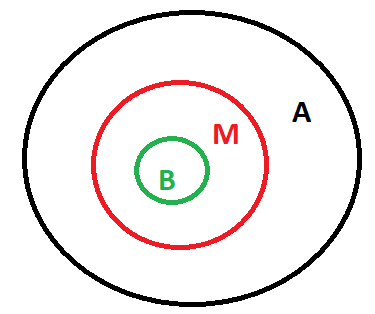
\includegraphics[scale=0.5]{S1DM3.png}

\end{frame}


\begin{frame}
	\titre{Exercices - schémas}

\begin{tabular}{lc}
2$^{\grave{e}me}$ syllogisme & Certains M sont A \\
		& Certains B ne sont pas M \\
\cline{2-2}
		& Certains B ne sont pas A \\
\end{tabular}
\pause

Pas valide : \pause\newline
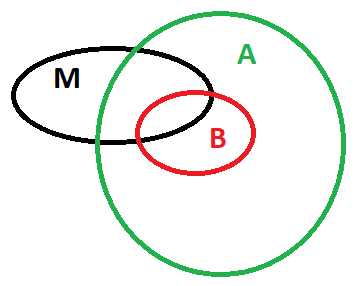
\includegraphics[scale=0.5]{S2DM3.png}

\end{frame}


\begin{frame}
	\titre{Exercices - schémas}

\begin{tabular}{lc}
3$^{\grave{e}me}$ syllogisme & Aucun M n'est A \\
		& Certains B sont M \\
\cline{2-2}
		& Certains B ne sont pas A \\
\end{tabular}
\pause
\textcolor{white}{lol}\newline

Valide : \pause La deuxième prémisse nous dit qu'il existe un individu qui est B et M, qu'on appellera $x$. \pause\newline

Or, la première prémisse nous dit que A et M sont des propriétés incompatibles. $x$, qui est déjà M, ne peut donc pas être A.\pause\newline

On a donc bien un individu, $x$, qui est B mais pas A
\end{frame}


\begin{frame}
	\titre{Exercices - schémas}

\begin{tabular}{lc}
4$^{\grave{e}me}$ syllogisme & Certains M sont A \\
		& Tous les B sont M \\
\cline{2-2}
		& Certains B ne sont pas A \\
\end{tabular}
\pause

Pas valide : \pause\newline
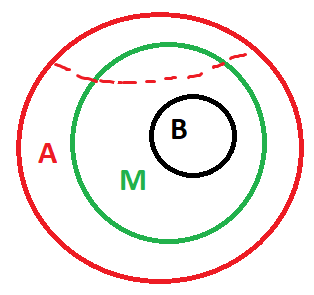
\includegraphics[scale=0.5]{S4DM3.png}

\end{frame}

